%%%%%%%%%%%%%%%%%%%%%%%%%%%%%%%%%%%%%%%%%%%%%%%%%%%%%%%%%%%%%%%%%%%%%%%%%%%%%%%%
\chapter{Introduction}
\label{ch:intro}
%%%%%%%%%%%%%%%%%%%%%%%%%%%%%%%%%%%%%%%%%%%%%%%%%%%%%%%%%%%%%%%%%%%%%%%%%%%%%%%%

In the last few years, the genomes of an increasing number of organisms have
been sequenced, generating a vast amount of information. Sequencing the genomes,
however, is just the first step in understanding these organisms at the
molecular level, and the focus has turned to understanding the function of genes
and other parts of the genome, as well as understanding their regulation at a
genome-wide scale, a field known as \emph{functional genomics}.

The central dogma of molecular biology states that the genetic information in
the DNA is \emph{transcribed} into portable messenger RNA (mRNA) molecules that
are subsequently \emph{translated} into proteins. While the DNA is viewed as a
storage device for genetic instructions, proteins actually execute these
instructions in several forms such as enzymes, transcription factors, structural
elements, immunoglobulins, hormones and signaling molecules.

A deoxyribonucleic acid (DNA) molecule is a repeating chain composed of four
different nucleotides: adenine (\tA), guanine (\tG), cytosine (\tC) and thymine
(\tT). DNA molecules are structurally organized in duplexes consisting of two
helical DNA molecules coiled around a common axis, forming a structure known as
the double helix. The messenger ribonucleic acid (mRNA) is a copy of a segment
of one DNA strand with uracil (\tU) replacing thymine (\tT). The basic building
blocks for the proteins are the amino acids. There are 22 amino acids naturally
occurring in plants, animals and bacteria. The sequence that forms a protein is
coded directly in the mRNA in terms of successive groups of three nucleotides
called \emph{codons}. The \emph{genes} are the RNA-encoding segments of the DNA,
and they are said to be \emph{expressed} in a cell when they are transcribed.
The set of all mRNA molecules, or transcripts, produced in one or a
population of cells is called \emph{transcriptome}.

To meet the challenge posed by functional genomics, new and highly ingenious
experimental techniques have been developed. Among them, microarrays have
emerged as the method of choice for large-scale gene expression studies because
they provide an efficient and rapid method to investigate the entire
transcriptome of a cell.

The complementary nature of the DNA double helix is the basis for the
large-scale measurement of mRNA levels with microarrays. Under the right
conditions, two complementary nucleic acid molecules (or \emph{strands}) combine
to form double stranded helices, a reaction know as \emph{hybridization}. This
principle allows the use of selected DNA strands with a known sequence of
nucleotides (the \emph{probes}) to query complex populations of unidentified,
complementary strands (the \emph{targets}).

%%%%%%%%%%%%%%%%%%%%%%%%%%%%%%%%%%%%%%%%%%%%%%%%%%%%%%%%%%%%%%%%%%%%%%%%%%%%%%%%
\section{High-density oligonucleotide microarrays}
\label{sec:intro_dnachip}

Several microarray technologies are available today, based on a variety of
fabrication techniques including printing with fine-pointed pins onto glass
slides, ink-jet printing, electrochemistry on microelectrode arrays and
photolithography. This thesis is mainly concerned with the production of
\emph{high-density oligonucleotide microarray}, sometimes called DNA chips,
that are fabricated by photolithography.

This type of microarray consists of relatively short DNA probes synthesized at
specific locations, called \emph{features} or \emph{spots}, of a solid surface.
Each probe is a single-stranded DNA molecule of 10 to 70 nucleotides that
perfectly matches with a specific part of a target molecule. The probes are used
to verify whether (or in which quantity) the targets are present in a given
biological sample.

The first step of a microarray experiment consists of collecting mRNAs or
genomic DNA from the cells or tissue under investigation. The mixture to be
analyzed is prepared with fluorescent tags and loaded on the array, allowing the
targets to hybridize with the probes. Any unbound molecule is washed away,
leaving on the array only those molecules that have found a complementary probe.
Finally, the array is exposed to a light source that induces fluorescence, and
an optical scanner reads the intensity of light emitted at each spot.

Under ideal conditions, each probe will hybridize only to its target.  Thus, it
is possible to infer whether a given molecule is present in the sample by
checking whether there is light coming from the corresponding spot of the array.
The expression level of a gene in a cell can also be inferred because each spot
contains several million identical probes, and the strength of the fluorescent
signal on a spot is expected to be proportional to the concentration of the
target in the sample. In practice, each target is queried by several probes
(called \emph{probe set}), and complex statistical calculations are performed to
infer the concentration from the observed signals.

Microarrays have been extensively used for cellular gene expression monitoring
and profiling \citep{Schena1995,Lockhart1996} with diverse applications such as
discovery of gene functions \citep{Cho1998,Hughes2000}, drug target
identification and validation \citep{Marton1998,Liotta2000}, analysis of drug
response \citep{Debouck1999}, classification of clinical samples
\citep{Perou1999} and detection of splicing variants \citep{Hu2001}. Microarrays
are also used for genotypic analysis, in two main areas: SNP analysis, and
mutation and variant detection. Single nucleotide polymorphisms (SNP) are the
most common source of genetic variation and, in fact, large numbers of SNPs have
been discovered using microarrays \citep{Lindblad-Toh2000}. Special mutation
detection arrays have also been used, for instance, to identify HIV variants
\citep{Kozal1996}.

The advantage of high-density oligonucleotide microarrays is that thay can have
more than a million spots, and are thus able to query tens of thousands of
genes, possibly covering the entire genome of an organism. This type of
microarray was originally designed in the late 1980s as a tool for DNA
sequencing, a technology that is known as Sequencing by Hybridization (SBH).
Today, the pioneering Affymetrix GeneChip\textR\ arrays, for instance, have up
to $6.5$ million spots on a coated quartz substrate measuring a little over
1~cm$^2$. The spots are as narrow as 5~$\mu$m (5~microns, or 0.005 mm), and are
arranged in a regularly-spaced rectangular grid \citep{McGall2002}.

\subsection{Photolithography}

GeneChip arrays are produced by combinatorial chemistry and techniques derived
from micro-electronics and integrated circuit fabrication. Probes are typically
25 bases long and are synthesized on the chip, in parallel, in a series of
repetitive steps. Each step appends the same kind of nucleotide to probes of
selected regions of the chip. The sequence of nucleotides added in each step is
called \emph{deposition sequence} or \emph{synthesis schedule}. The selection of
which probes receive the nucleotide is achieved by photolithography
\citep{Fodor1991,Fodor1993,Lipshutz1999}.

\begin{figure}[t]\centering
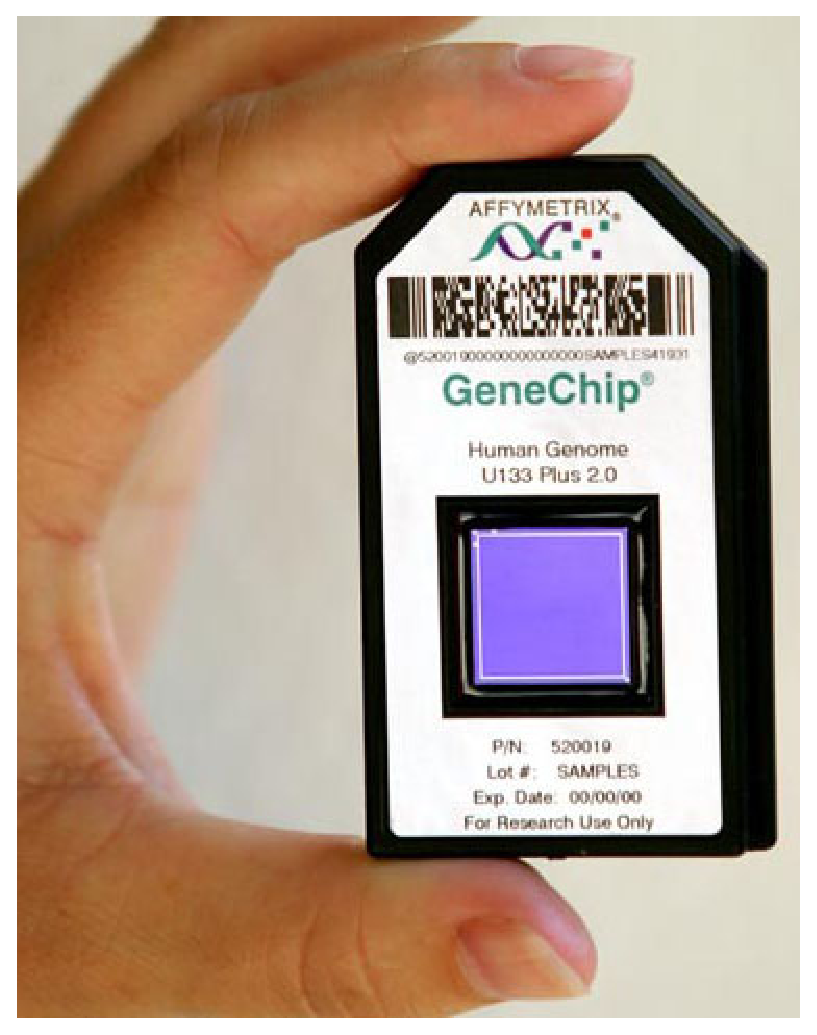
\includegraphics[width=.38\textwidth]{genechip.eps}
\hfill
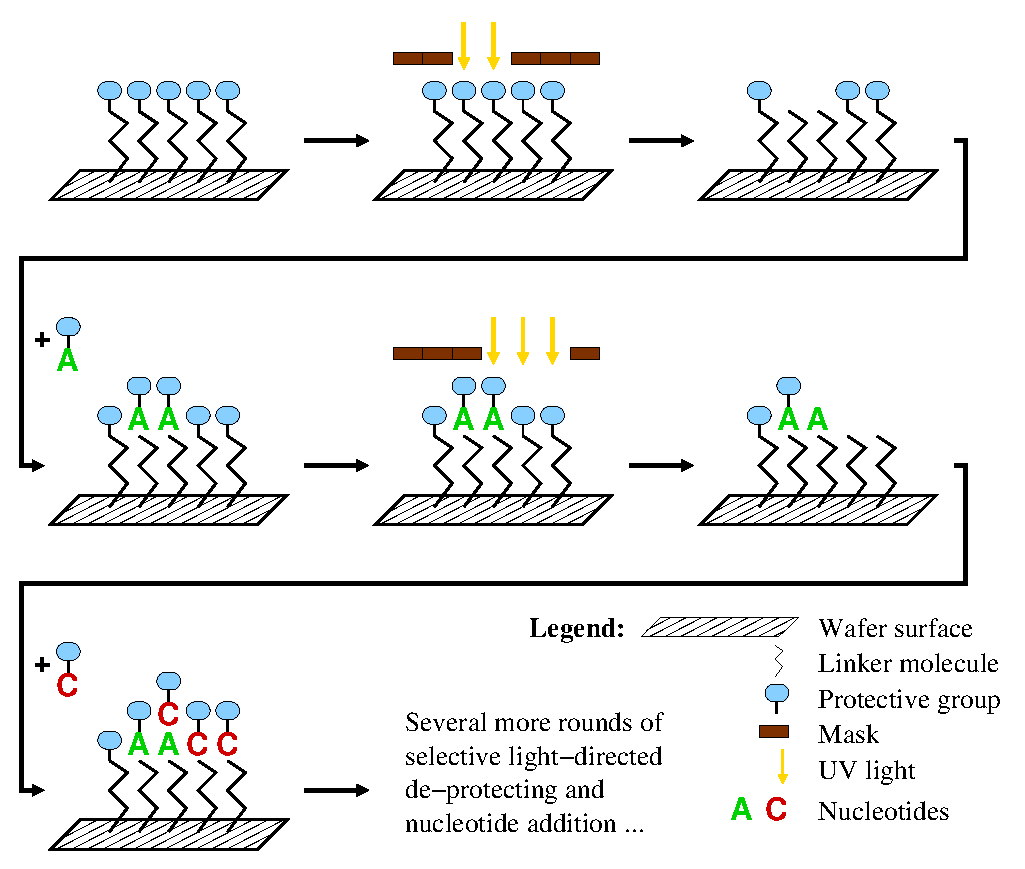
\includegraphics[width=.58\textwidth]{production.eps}
\caption{Left: Affymetrix GeneChip array (image courtesy of Affymetrix, Inc.).
  Right: probe synthesis via photolithographic masks. The chip is coated with a
  chemical compound and a light-sensitive protecting group; masks are used to
  direct light and activate selected probes for chemical coupling; nucleotides
  are appended to deprotected probes; the process is repeated until all probes
  have been fully synthesized.}
\label{fig:photolithography}
\end{figure}

Figure~\ref{fig:photolithography} illustrates this process: The quartz wafer of
a GeneChip array is initially coated with a chemical compound topped with a
light-sensitive protecting group that is removed when exposed to ultraviolet
light, activating the compound for chemical coupling. A lithographic mask is
used to direct light and remove the protecting groups of only those positions
that should receive the nucleotide of a particular synthesis step.  A solution
containing adenine (\tA), thymine (\tT), cytosine (\tC) or guanine (\tG) is then
flushed over the chip surface, but the chemical coupling occurs only in those
positions that have been previously deprotected. Each coupled nucleotide also
bears another protecting group so that the process can be repeated until all
probes have been fully synthesized.

Photolithographic masks are notoriously expensive and cannot be changed once
they have been manufactured. Thus, any change in the chip layout requires the
production of a new set of masks. A similar method of \emph{in situ} synthesis
known as Maskless Array Synthesizer (MAS) was later developed to eliminate the
need of such masks \citep{Singh-Gasson1999}. Probes are still built by repeating
cycles of deprotection and chemical coupling of nucleotides. The illumination,
however, relies on an array of miniature mirrors that can be independently
controlled to direct or deflect the incidence of light on the chip.

NimbleGen Systems, Inc.\ currently uses its Maskless Array Synthesizer (MAS)
technology based on its own Digital Micromirror Device (DMD) similar to Texas
Instruments' Digital Light Processor (DLP) that can control 786\,000 to $4.2$
million individual pixels of light to produce microarrays with spots as small as
16 $\mu$m $\times$ 16 $\mu$m \citep{Nuwaysir2002}. The {\sffamily geniom}\textR\
system of febit biotech GmbH, a highly-automated self-contained platform for
customized microarray production, also uses a micromirror array to direct the
synthesis process \citep{Baum2003}. Recently, the same technology has also been
used to synthesize arrays of peptides using 20 natural amino acids as well as
synthetic amino acid analogs \citep{Pellois2002,Gao2003,Li2004,Bhushan2006}.

\subsection{The unintended illumination problem}

Regardless of which method is used to direct light (masks or micromirror
arrays), it is possible that some probes are accidentally activated for chemical
coupling because of light diffraction, scattering or internal reflection on the
chip surface. This unwanted illumination of regions introduces unexpected
nucleotides that change probe sequences, significantly reducing their chances of
successful hybridization with their targets. Moreover, these faulty probes may
also introduce cross-hybridizations, which can interfere in the experiments
performed with the chip.

This problem is more likely to occur near the borders between a masked and an
unmasked spot (in the case of maskless synthesis, between a spot that is
receiving light and a spot that is not). This observation has given rise to the
term \emph{border conflict}.

It turns out that by carefully designing the \emph{arrangement} of the probes on
the chip and their \emph{embeddings} (the sequences of masked and unmasked steps
used to synthesize each probe), it is possible to reduce the risk of unintended
illumination. This issue becomes even more important as there is a need to
accommodate more probes on a single chip, which requires the production of spots
at higher densities and, consequently, with reduced distances between probes.

The main focus of this thesis is to design the layout of a microarray in such a
way that we minimize the incidence of the unintended illumination problem, what
we call the \emph{microarray layout problem} (MLP). Our goal is to study the
several phases of the design in detail, and to provide better and faster
algorithms for each phase. The MLP is discussed in Chapters \ref{ch:mlp} to
\ref{ch:affy}. A related problem is the \emph{shortest deposition sequence
problem}, which attempts to find the shortest deposition sequence to synthesize
a given set of probes. In Chapter \ref{ch:scs}, we analyze the feasibility of
finding an exact solution to this problem.

%%%%%%%%%%%%%%%%%%%%%%%%%%%%%%%%%%%%%%%%%%%%%%%%%%%%%%%%%%%%%%%%%%%%%%%%%%%%%%%%
\section{Manufacturing and design problems}
\label{sec:intro_problems}

We conclude this chapter by briefly describing other interesting mathematical
and computational problems that arise in the design and production of
oligonucleotide microarrays. Recently, \citet{Kahng2003b,Kahng2006} and
\citet{Atlas2004} proposed methodologies to integrate the various steps in the
design of a microarray chip, including probe selection, deposition sequence
design and, ultimely, layout design.

\paragraph{Probe selection.} Although a probe should only hybridize to its
target, it is known that, in practice, cross-hybridizations are likely to occur.
The goal of the probe selection problem is to find the smallest number of probes
with the specified length covering all genes of interest satisfying the three
criteria: homogeneity, sensitivity and specificity as proposed by
\citet{Lockhart1996}. Homogeneity ensures that probes can hybridize to their
targets at about the same experimental temperature. Sensitivity detects
self-complementarity and prevents probes with secondary structures. Specificity
ensures that probes are unique to each gene and eliminates probes that could
cross-hybridize.

This problem has been extensively studied in the past few years
\citep{Li2001,Kaderali2002,Rahmann2004}, and many algorithms have been proposed
to speed up the specificity check, regarded as the most computationally intensive
step \citep{Rahmann2002,Sung2003,Chou2004}. Among the presented approaches,
\citet{Rahmann2002} proposed a fast algorithm based on suffix arrays
\citep{Manber1990} that eliminates candidates that have a long common factor
with other genes.

\paragraph{Mask decomposition problem.} Once the probes have been selected and
the layout of the chip has been designed, the photolithographic masks must be
produced. The masks used by Affymetrix are fabricated by a series of
``flashes'', with each flash producing a rectangular part of the mask. The cost
of a mask is directly proportional to the number of flashes
\citep{Hubbell1998,Hubbell1999} and, in fact, there may be a limit in the number
of flashes before a more expensive fabrication technology must be used. Ideally,
each mask must be decomposed in the minimum number of rectangles in order to
reduce costs and incidence of errors.

\citet{Hannenhalli2002} studied this problem, called \emph{mask decomposition
problem}, as an instance of the rectilinear polygon interior cover problem,
which, according to \citet{Garey1979} was first shown to be NP-hard by
\citet{Masek}. Although approximation algorithms with small performance ratios
are known \citep{Franzblau1986}, \citet{Hannenhalli2002} explored the particular
characteristics of photolithographic masks to devise an efficient algorithm
which found provably optimal decompositions for a set of relatively small
GeneChip arrays.

\paragraph{Probe quality control.} During the production of a microarray chip,
it is possible that one synthesis step may be entirely compromised, resulting in
damages to all probes that receive the nucleotide of that particular step, and,
consequently, invalidating any experimental result obtained with the chip. In
order to detect such failures, Affymetrix have introduced the idea of producing a
set of \emph{quality control probes} (QC) on their chips \citep{Affymetrix2002}.
Target molecules for each QC probe are deliberately added to the biological
mixture during the experiment with the chip. If no synthesis step fails, the QC
probes should exhibit similar signal intensities. Thus, by measuring the
fluorescent signal emitted by each QC probe, it is possible to infer if they
have been correctly synthesized or not.

In fact, several copies of each quality control probe are produced on different
spots of the chip using different synthesis schedules (embeddings) in such a way
that it is possible to check if a synthesis step was compromised
\citep{Hubbell1999a} (and maybe even identify systematic problems in the chip
production). However, the validation proposed by \citet{Hubbell1999a} does not
take into account possible defects on isolated spots containing QC probes caused
by other manufacturing problems. For this reason, robust schemes based on a
combinatorial design approach that guarantee coverage of all synthesis steps and
that are able to tolerate a great number of unreliable QC probes have been
proposed \citep{Alon2001,Sengupta2002,Colbourn2002,Khan2003}.
